%& C:\Users\NAGARAJ\AppData\Roaming\TikzEdt\TikzEdt\023~1.0\TEMP_H~1
\begin{document}

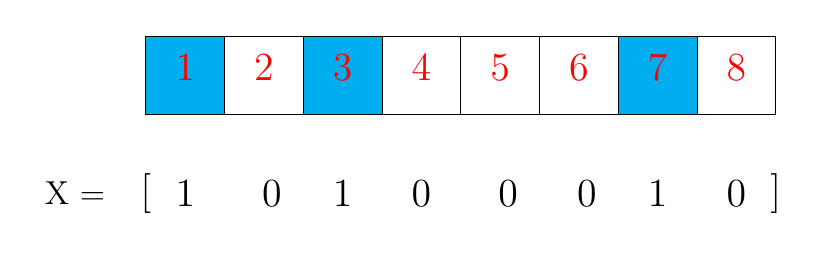
\begin{tikzpicture}


\draw [ fill=cyan] (-4,2) rectangle (-3,1);
\draw [] (-3,2) rectangle (-2,1);
\draw [fill=cyan] (-2,2) rectangle (-1,1);
\draw [] (-1,2) rectangle (0,1);
\draw [] (0,2) rectangle (1,1);
\draw  (1,2) rectangle (2,1);
\draw  [fill=cyan] (2,2) rectangle (3,1);
\draw (3,2) rectangle (4,1);
\node at (-4.9,0) {\large X = };




\node at (-3.5,1.6) {\Large \color{red}1};
\node at (-2.5,1.6) {\Large \color{red} 2};
\node at (-1.5,1.6) {\Large \color{red} 3};
\node at (-0.5,1.6) {\Large \color{red} 4};
\node at (0.5,1.6) {\Large \color{red} 5};
\node at (1.5,1.6) {\Large \color{red} 6};
\node at (2.5,1.6) {\Large \color{red} 7};
\node at (3.5,1.6) {\Large \color{red} 8};


\node at (-3.5,0) {\Large 1};
\node at (-2.4,0) {\Large 0};
\node at (-1.5,0) {\Large 1};
\node at (0.6,0) {\Large 0};
\node at (-0.5,0) {\Large 0};

\node at (1.6,0) {\Large 0};
\node at (2.5,0) {\Large 1};
\node at (3.5,0) {\Large 0};
\node at (-4,0) {\Large [};
\node at (4,0) {\Large ]};

\usetikzlibrary{calc}
\pgftransformreset
\node[inner sep=0pt,outer sep=0pt,minimum size=0pt,line width=0pt,text width=0pt,text height=0pt] at (current bounding box) {};
%add border to avoid cropping by pdflibnet
\foreach \border in {0.1}
  \useasboundingbox (current bounding box.south west)+(-\border,-\border) rectangle (current bounding box.north east)+(\border,\border);
\newwrite\metadatafile
\immediate\openout\metadatafile=\jobname_BB.txt
\path
  let
    \p1=(current bounding box.south west),
    \p2=(current bounding box.north east)
  in
  node[inner sep=0pt,outer sep=0pt,minimum size=0pt,line width=0pt,text width=0pt,text height=0pt,draw=white] at (current bounding box) {
\immediate\write\metadatafile{\p1,\p2}
};
\immediate\closeout\metadatafile
\end{tikzpicture}

\end{document}
